\documentclass[10pt]{article}

\usepackage[utf8]{inputenc}
\usepackage[T1]{fontenc}
\usepackage{lmodern}
\usepackage{amsmath,amssymb}
\usepackage{xcolor}
\usepackage{geometry}
\usepackage{array}
\usepackage{graphicx}

\geometry{paperwidth=16cm,paperheight=9cm,margin=0.75cm}
\pagestyle{empty}
\setlength{\parindent}{0pt}
\setlength{\parskip}{0.12cm}

\definecolor{DeepBlue}{RGB}{18,45,83}
\definecolor{AccentBlue}{RGB}{35,111,190}
\definecolor{Gold}{RGB}{236,178,46}
\definecolor{DarkGray}{RGB}{58,65,76}
\definecolor{LightGray}{RGB}{245,247,250}

\newcommand{\slide}[2]{%
  \clearpage
  {\color{DeepBlue}\Large\bfseries #1}\par
  \vspace{0.08cm}
  {\color{AccentBlue}\rule{4.1cm}{0.04cm}}\par
  \vspace{0.22cm}
  #2
  \vfill
  \noindent\makebox[0pt][l]{\hspace*{-0.72cm}\raisebox{-0.36cm}[0pt][0pt]{
\includegraphics[width=2.35cm]{qf_logo.jpg}}}\hfill{\scriptsize\color{DarkGray}\thepage}
}

\newcommand{\titleslide}[3]{%
  \clearpage
  \vspace*{1.35cm}
  \begin{center}
    {\color{DeepBlue}\Huge\bfseries #1}\par
    \vspace{0.35cm}
    {\color{DarkGray}\large #2}\par
    \vspace{0.55cm}
    {\color{AccentBlue}\rule{9cm}{0.05cm}}\par
    \vspace{0.9cm}
    {\color{DarkGray}#3}\par
  \end{center}
}

\newcommand{\keyword}[1]{\textcolor{AccentBlue}{\textbf{#1}}}
\newcommand{\important}[1]{\textcolor{DeepBlue}{\textbf{#1}}}
\newcommand{\boxformula}[1]{%
  \[
    \boxed{#1}
  \]
}

\begin{document}

\titleslide
{Calcul de SLOIM : scénarios historiques et hypothétiques}
{Utilisation de l'ACP/PCA pour construire des stress de courbe ZC fiables et interprétables}
{Quant Factory -- Juin 2026}

\slide{Chaîne de calcul visée}{
La SLOIM arrive après le calcul du PnL stressé. Le moteur peut rester le même : ce qui change, c'est l'ensemble de scénarios injecté en entrée.

\boxformula{
\text{Scénario de stress}
\rightarrow
PnL_i^{(s)}
\rightarrow
L_i^{(s)}
\rightarrow
SLOIM_i^{(s)}
}

\begin{itemize}
  \item Le scénario choque la courbe ZC ou les facteurs de risque.
  \item Le portefeuille du membre est revalorisé sous ce choc.
  \item Le PnL est transformé en perte stressée positive.
  \item La perte est comparée à l'IM pour obtenir la SLOIM.
\end{itemize}
}

\slide{Deux familles de scénarios pour le PnL stressé}{
Le coeur du travail est le suivant : pour calculer la SLOIM, on doit d'abord calculer un \keyword{PnL stressé} pour chaque membre compensateur.

\vspace{0.15cm}

Ce PnL stressé sera calculé sous deux familles de scénarios :

\begin{itemize}
  \item des \keyword{scénarios historiques stressés}, construits à partir de mouvements réellement observés ;
  \item des \keyword{scénarios hypothétiques}, construits par ACP/PCA à partir de la structure statistique de la courbe ZC.
\end{itemize}
}

\slide{Premier type : scénarios historiques stressés}{
Les scénarios historiques stressés rejouent des mouvements de marché déjà observés sur la courbe ZC.

\begin{itemize}
  \item Ils ont l'avantage d'être réalistes : ils proviennent de données effectivement observées.
  \item Ils permettent de garder une cohérence entre les piliers de la courbe.
  \item Ils sont directement utilisables dans le moteur de PnL stressé.
\end{itemize}

\vspace{0.2cm}

Limite principale : ils ne testent que les stress présents dans l'historique. Un choc plausible mais jamais observé dans la fenêtre retenue ne sera pas couvert.
}

\slide{Deuxième type : scénarios hypothétiques ACP}{
Pour compléter les scénarios historiques, on construit des scénarios hypothétiques à l'aide de l'ACP/PCA.

\begin{itemize}
  \item L'ACP apprend la structure des mouvements historiques de la courbe ZC.
  \item Elle extrait les directions qui expliquent le plus de variance dans les données.
  \item Elle permet de créer des chocs extrêmes mais cohérents avec les comportements observés.
\end{itemize}

\vspace{0.2cm}

L'ACP sert donc à éviter des stress arbitraires : on construit les chocs hypothétiques à partir de la variance réelle des données.
}

\slide{La matrice de données utilisée par l'ACP}{
On part d'une matrice $X$ de mouvements historiques de la courbe ZC.

\begin{itemize}
  \item Les lignes représentent les dates historiques.
  \item Les colonnes représentent les piliers de maturité de la courbe ZC.
  \item Les valeurs sont des returns ou variations de prix ZC, centrés avant ACP.
\end{itemize}

\boxformula{
\Sigma
=
\frac{1}{N-1}X^\top X,
\qquad
\Sigma v_k = \lambda_k v_k
}

\begin{itemize}
  \item $v_k$ : direction principale de mouvement de la courbe.
  \item $\lambda_k$ : variance expliquée par cette direction.
\end{itemize}
}

\slide{PC1, PC2 et PC3 : interprétation économique}{
En taux, les trois premières composantes principales sont généralement les plus importantes.

\begin{itemize}
  \item \keyword{PC1 -- niveau} : toute la courbe monte ou baisse globalement.
  \item \keyword{PC2 -- pente} : les maturités courtes et longues bougent en sens différent.
  \item \keyword{PC3 -- courbure} : le ventre de courbe bouge différemment des extrémités.
\end{itemize}

\vspace{0.2cm}

Cette interprétation vient de la forme des vecteurs propres. Elle est classique dans la littérature taux, notamment chez Litterman et Scheinkman, mais elle doit être vérifiée sur nos propres données.
}

\slide{Effet des facteurs sur la courbe}{
\vspace{-0.15cm}
\begin{center}
  \includegraphics[width=6.7cm]{yield_curve_impact_litterman.png}
\end{center}

\vspace{-0.25cm}
{\scriptsize\color{DarkGray}\textit{Source : Litterman \& Scheinkman (1991).}}
}

\slide{Pourquoi retenir principalement les trois premiers facteurs ?}{
L'intérêt de l'ACP est de réduire la dimension du problème sans perdre l'essentiel de l'information.

\begin{itemize}
  \item La courbe ZC contient beaucoup de piliers, donc beaucoup de facteurs de risque.
  \item Les premiers facteurs expliquent généralement la majorité de la variance historique.
  \item Retenir PC1, PC2 et PC3 permet de couvrir les mouvements dominants : niveau, pente et courbure.
  \item Les facteurs suivants expliquent souvent une part beaucoup plus faible et plus bruitée.
\end{itemize}

\vspace{0.2cm}

On obtient ainsi des scénarios plus simples, plus stables et plus faciles à justifier devant un superviseur ou une équipe risque.
}

\slide{Variance expliquée par les trois facteurs}{
\important{Moyenne :} trois facteurs expliquent \keyword{98.4\%} de la variance totale.

\begin{center}
  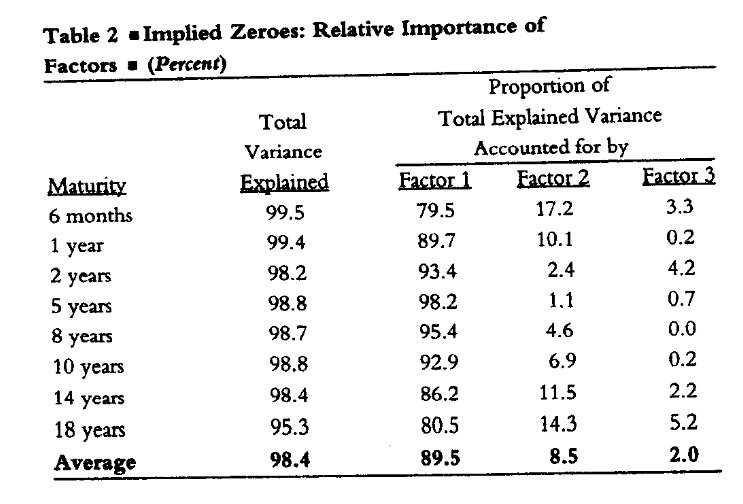
\includegraphics[width=6.2cm]{pca_variance_table.png}
\end{center}

\vspace{-0.2cm}
{\scriptsize\color{DarkGray}\textit{Source : Litterman \& Scheinkman (1991).}}
}

\slide{Lecture de la formule de stress ACP}{
La formule ACP reconstruit un choc complet de courbe à partir des facteurs principaux.

\boxformula{
\Delta r_{\mathrm{stress}}
=
\sum_{k=1}^{K}
m_k \sqrt{\lambda_k}\, v_k
}

\begin{itemize}
  \item $\Delta r_{\mathrm{stress}}$ est un \keyword{vecteur} de choc sur tous les piliers ZC.
  \item $v_k$ est le vecteur propre : il donne la forme du facteur $PC_k$.
  \item $\sqrt{\lambda_k}$ est l'écart-type du facteur, donc sa volatilité historique.
  \item $m_k$ indique combien d'écarts-types on applique au facteur.
  \item $K$ est le nombre de facteurs retenus ; dans notre cas cible, $K=3$ avec PC1, PC2 et PC3.
\end{itemize}
}

\slide{Construction d'un choc hypothétique ACP}{
Une fois les facteurs identifiés, on construit un choc de courbe en appliquant des multiplicateurs extrêmes aux composantes principales.

\boxformula{
\Delta r_{\mathrm{stress}}
=
\sum_{k=1}^{K}
m_k \sqrt{\lambda_k}\, v_k
}

Exemple :

\boxformula{
\mathrm{Stress}
=
4\sigma_1 v_1
-
3\sigma_2 v_2
+
2\sigma_3 v_3
}

Cela signifie : choc fort sur le niveau, choc inverse sur la pente et choc de courbure. Le résultat est un mouvement complet de courbe, défini sur tous les piliers ZC.
}

\slide{Comment choisir les multiplicateurs $m_k$ ?}{
Les $m_k$ sont essentiels : ils déterminent l'intensité du stress appliqué à chaque facteur.

\begin{itemize}
  \item \keyword{Choix expert} : définir un choc volontairement sévère, par exemple $m_1=4$, $m_2=-3$, $m_3=0$.
  \item \keyword{Quantiles historiques} : calculer les scores ACP historiques, puis prendre des quantiles extrêmes.
  \item \keyword{Analyse de sensibilité} : tester plusieurs combinaisons de niveau, pente et courbure.
\end{itemize}

\vspace{0.15cm}

Même si PC1 explique le plus de variance, PC2 et PC3 restent importants car ils capturent des formes de risque différentes. Certains portefeuilles peuvent être plus sensibles à la pente ou à la courbure qu'au niveau global.
}

\slide{Interprétation du signe des $m_k$}{
Le signe de $m_k$ donne le sens du choc appliqué au facteur $PC_k$.

\begin{itemize}
  \item $m_k>0$ : on applique le facteur dans le sens du vecteur $v_k$.
  \item $m_k<0$ : on applique le facteur dans le sens opposé.
  \item Pour PC1, cela correspond à un choc global de niveau dans un sens ou dans l'autre.
  \item Pour PC2, cela inverse le sens du mouvement de pente.
  \item Pour PC3, cela inverse le sens du mouvement de courbure.
\end{itemize}

\vspace{0.15cm}

Point important : le signe d'un vecteur propre est arbitraire. Il faut donc toujours visualiser $PC_1$, $PC_2$ et $PC_3$ avant d'interpréter ce que signifie un $m_k$ positif ou négatif.
}

\slide{Utilisation finale dans le moteur SLOIM}{
Les scénarios hypothétiques ACP ne changent pas la formule de SLOIM. Ils changent uniquement les stress utilisés pour calculer les PnL.

\boxformula{
\{\text{Stress historiques}\}
\cup
\{\text{Stress ACP hypothétiques}\}
\rightarrow
PnL^{(s)}
\rightarrow
SLOIM^{(s)}
}

\begin{itemize}
  \item Les stress historiques apportent le réalisme empirique.
  \item Les stress ACP apportent des chocs extrêmes, structurés et interprétables.
  \item Les deux familles permettent d'obtenir une SLOIM plus robuste.
  \item Le Cover-2 est ensuite calculé sur l'ensemble du set de stress.
\end{itemize}
}

\slide{Sources et prochaines étapes}{
\begin{itemize}
  \item \keyword{Litterman \& Scheinkman (1991)} -- \textit{Common Factors Affecting Bond Returns}. Référence sur les facteurs niveau, pente et courbure.
  \item \keyword{Note fonds de défaut QF}. Cadre SLOIM, Cover-2 et allocation des contributions.
  \item \keyword{Références CCP / EMIR}. Fonds de défaut et contributions proportionnelles aux expositions.
\end{itemize}

\vspace{0.2cm}

Prochaine étape : implémenter les stress ACP dans le notebook, comparer la SLOIM historique et la SLOIM hypothétique, puis mesurer l'impact sur le fonds Cover-2 et son allocation.
}

\end{document}
